\section{Evaluation} \label{sec:experiment}
We carried out our evaluation on a desktop PC running Ubuntu 10.04 with a Core i5, 2530 Mhz processor, and 4 GB of RAM. 
We have implemented a tool, called \CodeIn{PolicySplitter} to split policies according to a given splitting criterion automatically.
The tool is implemented in Java and is available for download \cite{splitter}.

\subsection{Objectives and Metrics}
Our evaluation intends to answer the following research questions:
\begin{enumerate}
\item \textbf{RQ1.} How faster can request processing time of multiple Sun PDPs with policies split by our approach achieve compared
to an existing single Sun PDP? This question helps show that our approach can improve performance in terms of request processing time. 
Moreover, we compare request processing time for different splitting criteria.
\item \textbf{RQ2.} With comparable PDP policy sizes? Is the system more performant when the architecture is synergic? 
This research question, questioned in Section \ref{sec:context}, investigates \textit{Hypothesis 2}.
\item \textbf{RQ3.} How faster does request processing time of XEngine achieve compared
to that of Sun PDP for both a single policy and policies split by our approach?
This question helps show that our approach can improve performance in terms of request processing time for other advanced policy evaluation 
engines such as XEngine.
\item \textbf{RQ4.} The bigger the PDP policy size, do we observe higher slope of the execution time with an increasing workload? This research question investigates \textit{Hypothesis 1} 
(mentioned in Section \ref{sec:context}) on the impact of the number of rules in a given PDP on system response.
\end{enumerate}

To address these research questions, we go through the following evaluation setup based on two different empirical studies:
\begin{itemize}
\item First, we evaluate the performance improvement regarding the decision making process by taking into consideration the whole system 
(PEPs and PDPs). We compared request processing time with a single global policy (handled by a single PDP) against request processing time with
split policies. All the splitting criteria have been considered in our evaluation.
\CodeIn{IA} denotes an ``Initial Architecture'', which uses the single global policy for request processing. 
This step allows studying the behavior of splitting criteria that preserve the synergy property in the access control architecture.

\item Second, we evaluate the performance of PDPs in isolation to compare the splitting criteria independently from the system.
Recall that in this step, we do not reason about the synergy property since we don't consider the application level.
We replace Sun PDPs with a request evaluation engine XEngine \cite{Xengine}. The objective of this evaluation is to investigate how our approach impacts performance for subjects combined with XEngine.
\end{itemize}

\subsection{Subjects}
The subjects include three real-life Java systems each of which interacts with access control policies. 
Full details on our subjects are available in \cite{evaluation}. We next describe our three subjects.
\begin{itemize}	
\item Library Management System (LMS) provides web services to manage books in a public library.
\item Virtual Meeting System (VMS) provides web conference services. VMS allows users to organize
online meetings in a distributed platform.
\item Auction Sale Management System (ASMS) allows users to buy or sell items online. A seller 
initiates an auction by submitting a description of an item that she wants to sell with its expected minimum 
price. Users then participate in the bidding process by
bidding the item. To bid on the item, user must have enough money in her account before bidding.
\end{itemize}
Our subjects are initially built upon Sun PDP \cite{sunxacml} as a decision engine, which is a popularly used PDP to evaluate requests. We started by a processing step, in which we have augmented the rules number 
in the three original policies for these studies, as it would be difficult to observe a performance improvement results with systems including few rules. In our evaluations, LMS policy contains 720 rules, VMS has 
945 rules while ASMS implements 1760 rules. The rules that we added do not modify the system behavior as 
they are conform to the specifications. Moreover, to compare performance improvement over existing PDPs, we adopt XEngine (instead of Sun PDP) in our subjects to evaluate requests.
XEngine is an advanced policy evaluation engine, which transforms the hierarchical tree structure of the XACML policy to a flat structure to reduce request processing time. XEngine 
also handles various combining algorithms supported by XACML. 

\subsection{Performance Improvement: Sun PDP}\label{subsec:performanceimprovement}
In order to answer \textbf{RQ1}, we generated the resulting sub-policies for all the splitting criteria defined in 
Section~\ref{subsec:SplittingCriteria}.
For each splitting criterion, we have executed system tests to generate requests that trigger all the PEPs in the evaluation. 
The test generation step leads to the execution of all combinations of possible requests described in our previous work \cite{testcase}.  
The process of test generation is repeated ten times to alleviate the impact of randomness. We applied this process to each splitting criterion and calculated evaluation time on average of a system under test.
% We only consider the execution time of the PDP and we do not include the executions of the system functions. 
Figure \ref{fig:processing time} presents evaluation time for policies split
based on each splitting criterion and the global policy of subjects. We can make two observations:
\begin{itemize}
\item Compared to the evaluation time of \CodeIn{IA}, our approach improves performance for all of splitting criteria
in terms of evaluation time. This observation is consistent with our expected results; the evaluation time against
policies with a smaller number of rules (compared with the number of rules in \CodeIn{IA}) is faster than that against
policies in \CodeIn{IA}.
\item The splitting criterion \normalsize $SC=\langle Action, Resource\rangle$ enables to show the shortest evaluation time. 
Recall that the PEPs in the evaluation are scattered across different methods in a subject by a categorization 
based on $SC_{2}=\langle Resource,Action\rangle$. This observation pleads in favor of applying a splitting criterion 
that takes into account the PEP-PDP synergy.
\end{itemize}
 \begin{figure*}[h!]
  \centering
  \subfloat[LMS]{\label{fig:gull}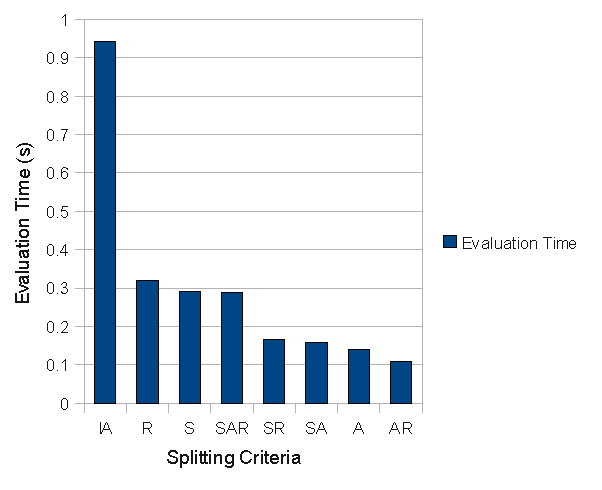
\includegraphics[width=0.33\textwidth]{LMS.pdf}}                
  \subfloat[VMS]{\label{fig:VMS}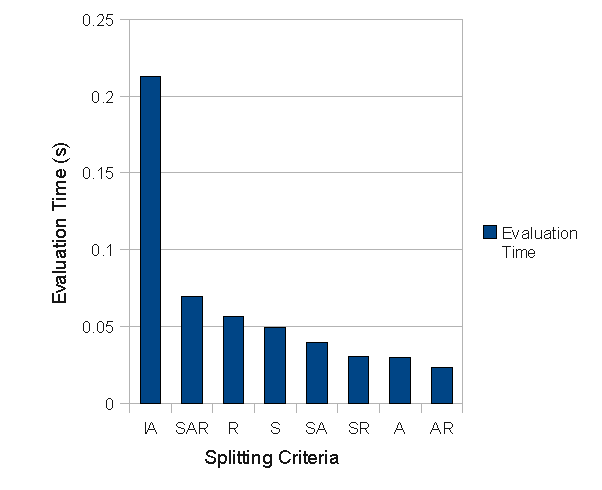
\includegraphics[width=0.33\textwidth]{VMS.pdf}}
  \subfloat[ASMS]{\label{fig:ASMS}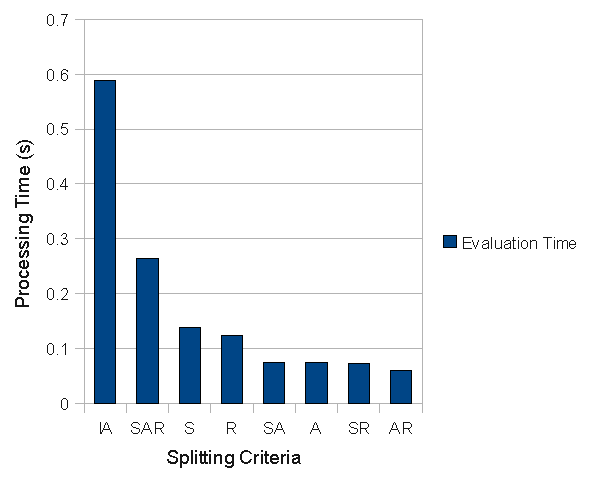
\includegraphics[width=0.33\textwidth]{ASMS.pdf}}
  \caption{Request Processing Time for the Three subjects}
  \label{fig:processing time}
\end{figure*}
 

To identify the splitting criterion that generates the smallest number of PDPs, we have studied the number of policies generated by the
 splitting. Figure \ref{pdpnumber} shows the results.
We observed the number of policies based on our proposed three categories: (1) the $SC_{1}$ category leads to the smallest number $N_1$ of PDPs, 
(2) the $SC_{2}$ category leads to a reasonable number
 $N_2$ ($N_1$<$N_2$<$N_3$) of PDPs, and (3) $SC_{3}$ leads to the largest number $N_3$ of PDPs.
While the $SC_{1}$ category leads to the smallest number of PDPs, each PDP encapsulates a relatively high number of rules in a policy (compared
with that of $SC_{2}$ and $SC_{3}$, which leads to performance degradation. 
\begin{figure}[!h]
\centering
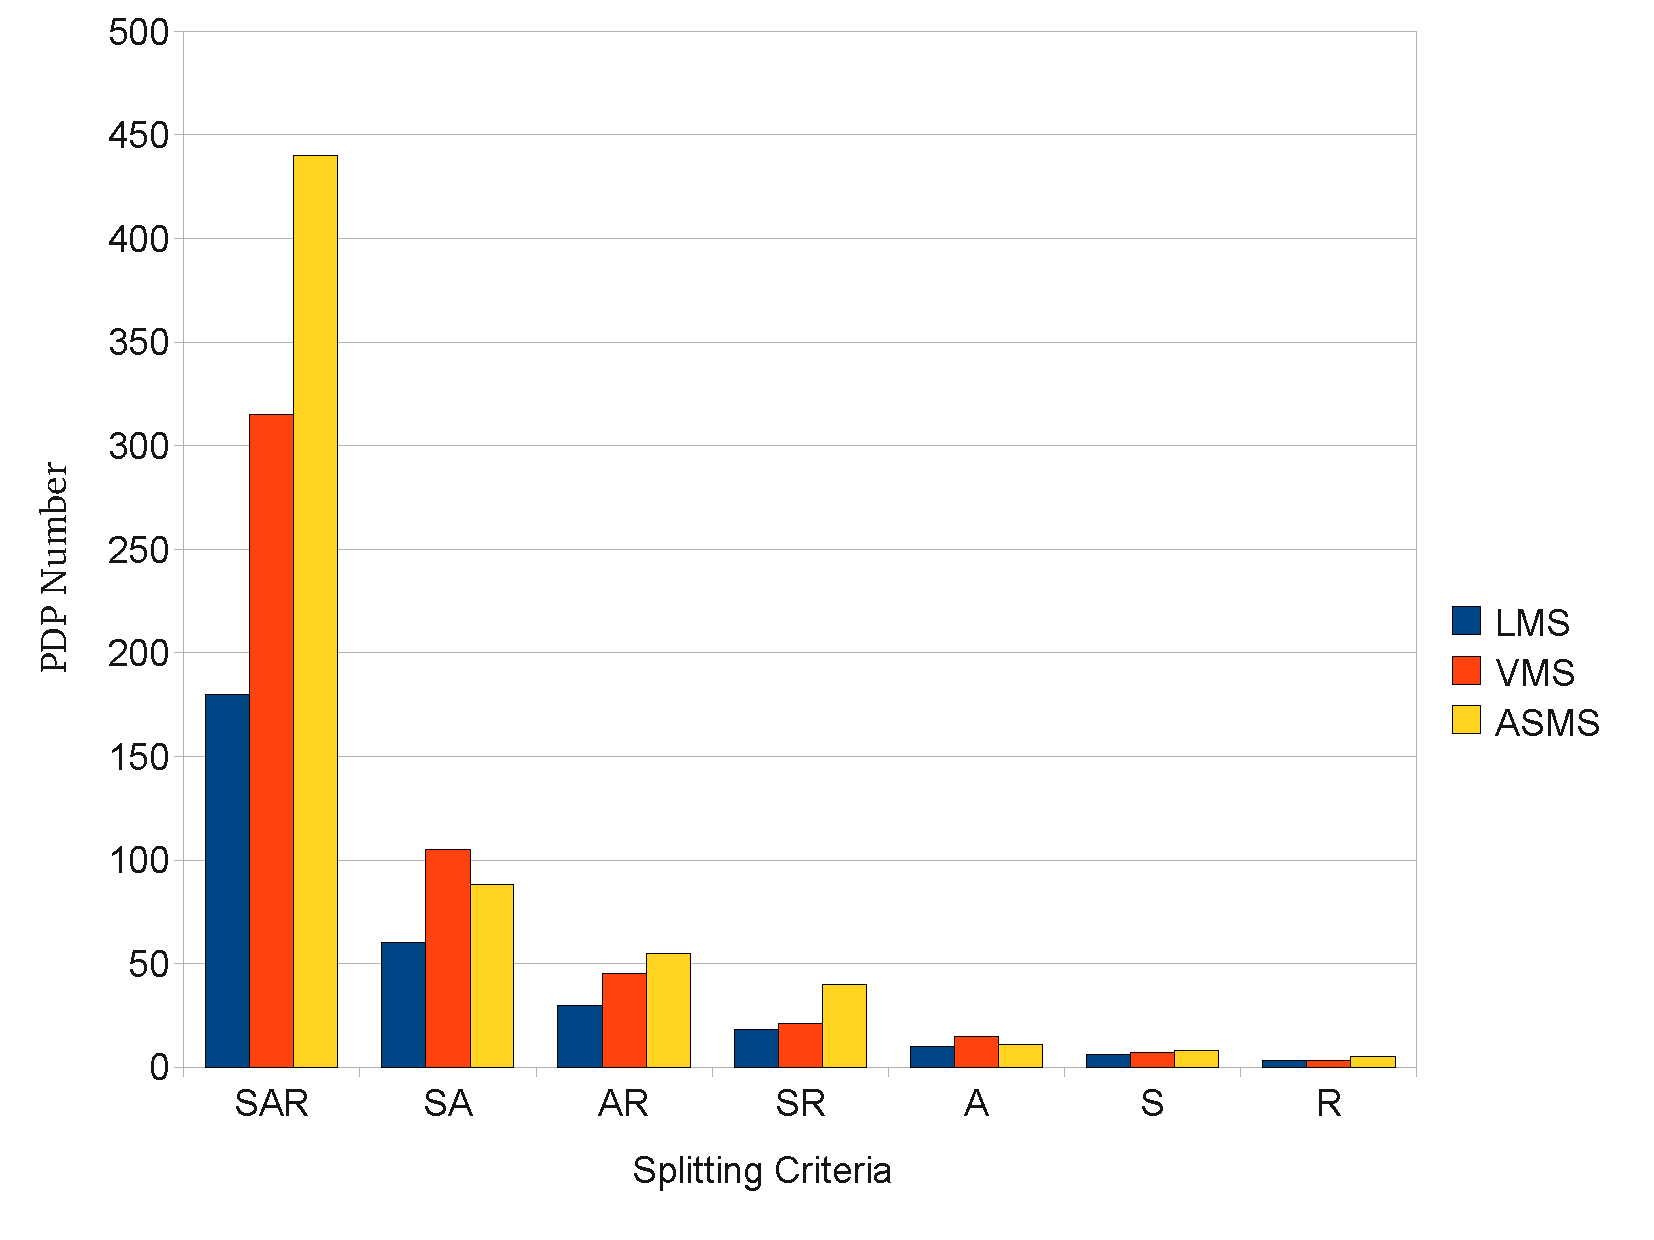
\includegraphics[width=8.5cm, height=7.2cm]{pdpnumber.pdf}
\begin{center}
\caption{PDP Number produced with Splitting Criteria}
\label{pdpnumber}
\end{center}
\end{figure}
We have classified splitting criteria according to their preservation of the synergy property considering our subjects. The classification is shown in Table \ref{Classification}. 
$AR$, $A$ and $R$ are synergic splitting criteria since all the PEPs in our considered three systems are organized as shown in Figure \ref{PEPdeploymentexample}. 
\begin{table}[t]
\centering
\begin{tabular}{|>{\tiny}c|>{\tiny}c|>{\tiny}c|>{\tiny}c|>{\tiny}c|>{\tiny}c|>{\tiny}c|>{\tiny}c|>{\tiny}c|}   
\hline  \rowcolor{black} \scriptsize \bf \textcolor {white}{}
& \scriptsize \bf \textcolor {white}{S}
& \scriptsize \bf \textcolor {white}{A}
& \scriptsize \bf \textcolor  {white}{R}
& \scriptsize \bf \textcolor  {white}{SA}
& \scriptsize \bf \textcolor  {white}{SR}
& \scriptsize \bf \textcolor  {white}{AR} 
& \scriptsize \bf \textcolor  {white}{SAR}
& \scriptsize \bf \textcolor {white}{IA}\\ \hline
\scriptsize  {Synergic}
&\scriptsize  {}
& \scriptsize {x}
& \scriptsize {x}
& \scriptsize {}
& \scriptsize {}
& \scriptsize {x}
& \scriptsize {}
& \scriptsize {x}
  \\ \hline
\scriptsize  {Not Synergic}
&\scriptsize  {x}
& \scriptsize {}
& \scriptsize {}
& \scriptsize {x}
& \scriptsize {x}
& \scriptsize {}
& \scriptsize {x}
& \scriptsize {}
  \\ \hline
\end{tabular}
\caption{Splitting Criterion Classification}
\label{Classification}
\end{table}

To answer \textbf{RQ2}, we have evaluated PDPs in the three systems and for the different splitting criteria. The results presented in Figure 
\ref{average} show the average number of rules in each PDP, for each splitting criterion in the three systems. We can observe that the $AR$ 
criterion produces comparable size of PDPs with the $SR$ criterion, however, as shown in Figure 
\ref{fig:processing time}, $AR$ is the best splitting criterion, in term of evaluation time performance. 
Moreover, the number of PDPs produced with the splitting critera $S$ and $A$ is comparable and the criterion $A$ which is synergic has evaluation 
time less than the one produced by the splitting criterion $S$ which is not synergic.
This result supports our hypothesis \textit{Hypothesis 2}, which states that with comparable PDP sizes, the overall system would 
be more performant when the architecture is synergic.

\begin{figure}[!h]
\centering
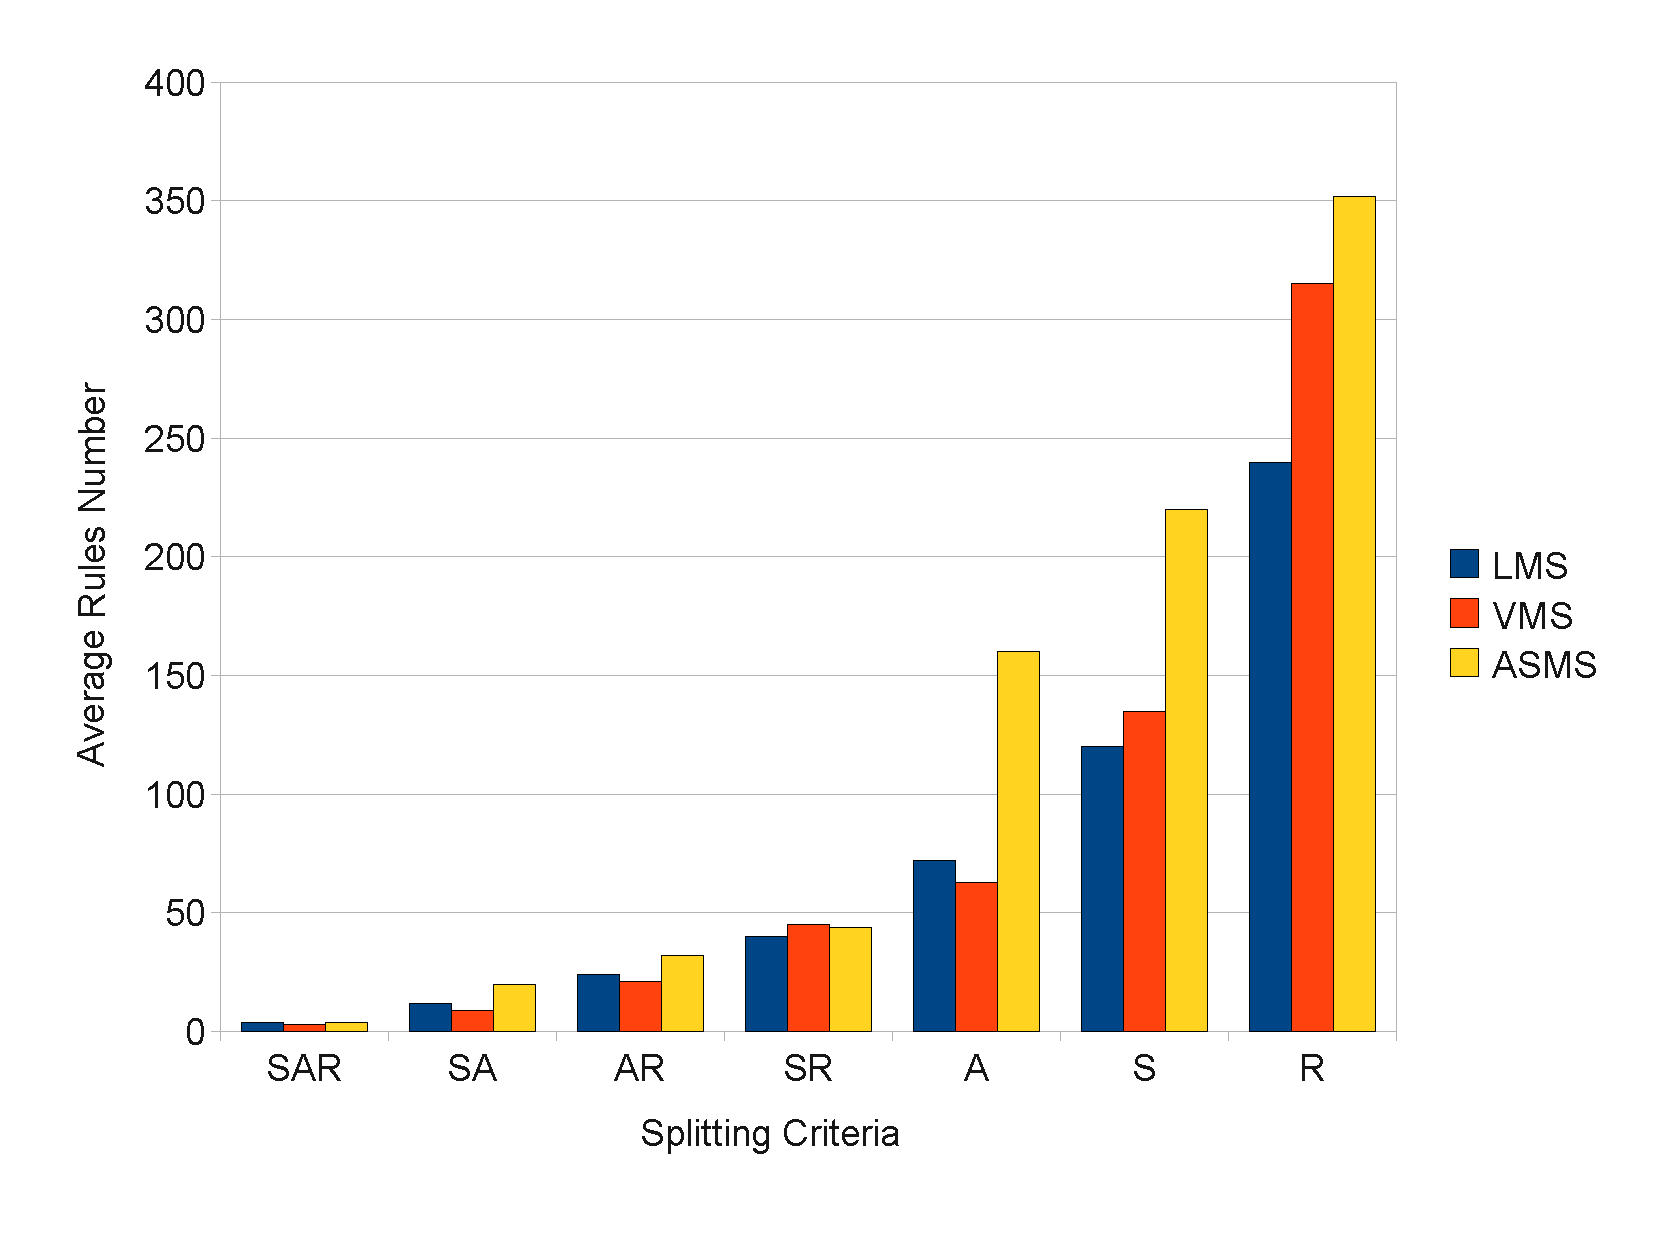
\includegraphics[width=8.5cm, height=7.2cm]{averagerules.pdf}
\begin{center}
\caption{Average of Rules Number/PDP in the Three Systems}
\label{average}
\end{center}
\end{figure}
\subsection{Performance Improvement: XEngine}
In order to answer \textbf{RQ3}, we measure request processing time of XEngine compared with that of Sun PDP
for policies split by our approach.
The goal of this empirical study is to show the impact of combining
XEngine with our splitting process. XEngine improves dramatically the performance of the PDP, mainly for
three reasons:
\begin{itemize}
\item It uses a refactoring process that transforms the hierarchical structure of the XACML policy to a flat structure.
\item  It converts multiple combining algorithms to single one.
\item  It relies on a tree structure that minimizes the request
processing time.
\end{itemize}
We propose to use XEngine conjointly with the refactoring process presented in this work. We have evaluated our approach in two settings:
\begin{itemize}
\item Considering evaluation with a decision engine based on Sun PDP with split policies and with the initial policy.
\item Considering evaluation with a decision engine based on XEngine with split policies and with the initial policy.
\end{itemize}
In this step, we do not reason about the synergy, since we do not consider the application level for the three systems. We measure request processing time by evaluating randomly generated set of 10,000 requests as proposed in our previous work \cite{request}.
The request time processing is evaluated for the three systems. The results bare presented in Tables \ref{table:LMSeval}, \ref{table:VMSeval} and \ref{table:ASMSeval} and enable to answer \textbf{RQ3}.
We observe that, when our subjects are equipped with XEngine, our proposed approach 
substantially improves performance (compared to the results with Sun PDP). For the splitting criteria SC=$\langle Action \rangle$,
in the LMS system, the evaluation time is reduced about 9 times: from 2703 ms to 290 ms with XEngine. This empirical 
observation pleads in favor of applying our proposed refactoring process with XEngine.
\begin{table}[t]
\centering
\begin{tabular}{|>{\tiny}c|>{\tiny}c|>{\tiny}c|>{\tiny}c|>{\tiny}c|>{\tiny}c|>{\tiny}c|>{\tiny}c|>{\tiny}c|}   
\hline  \rowcolor{black} \scriptsize \bf \textcolor {white}{}
& \scriptsize \bf \textcolor {white}{SAR}
& \scriptsize \bf \textcolor {white}{AR}
& \scriptsize \bf \textcolor  {white}{SA}
& \scriptsize \bf \textcolor  {white}{SR}
& \scriptsize \bf \textcolor  {white}{R}
& \scriptsize \bf \textcolor  {white}{S} 
& \scriptsize \bf \textcolor  {white}{A}
& \scriptsize \bf \textcolor {white}{IA}\\ \hline
\scriptsize  {Sun PDP }
&\scriptsize  {485}
& \scriptsize {922}
& \scriptsize {1453}
& \scriptsize {1875}
& \scriptsize {2578}
& \scriptsize {2703}
& \scriptsize {2703}
& \scriptsize {2625}
  \\ \hline
\scriptsize  {XEngine}
&\scriptsize  {26}
& \scriptsize {47}
& \scriptsize {67}
& \scriptsize {95}
& \scriptsize {190}
& \scriptsize {164}
& \scriptsize {120}
& \scriptsize {613}
  \\ \hline
\end{tabular}

\caption{Evaluation Time in LMS}
\label{table:LMSeval}
\vspace{5 mm}
%\end{table}
%\begin{table}[h!]
\centering
\begin{tabular}{|l|l|l|l|l|l|l|l|l|}   
\hline  \rowcolor{black} \scriptsize \bf \textcolor {white}{}
& \scriptsize \bf \textcolor {white}{SAR}
& \scriptsize \bf \textcolor {white}{AR}
& \scriptsize \bf \textcolor  {white}{SA}
& \scriptsize \bf \textcolor  {white}{SR}
& \scriptsize \bf \textcolor  {white}{R}
& \scriptsize \bf \textcolor  {white}{S} 
& \scriptsize \bf \textcolor  {white}{A}
& \scriptsize \bf \textcolor {white}{IA}\\ \hline
\scriptsize  {Sun PDP }
& \scriptsize  {1281}
& \scriptsize {2640}
& \scriptsize {3422}
& \scriptsize {3734}
& \scriptsize {6078}
& \scriptsize {5921}
& \scriptsize {6781}
& \scriptsize {5766}
  \\ \hline
\scriptsize  {XEngine}
& \scriptsize  {34}
& \scriptsize {67}
& \scriptsize {96}
& \scriptsize {145}
& \scriptsize {384}
& \scriptsize {274}
& \scriptsize {149}
& \scriptsize {265}
  \\ \hline
\end{tabular}

\caption{Evaluation Time in VMS}
\label{table:VMSeval}
\vspace{5 mm}
\centering
\begin{tabular}{|l|l|l|l|l|l|l|l|l|}   
\hline  \rowcolor{black} \scriptsize \bf \textcolor {white}{}
& \scriptsize \bf \textcolor {white}{SAR}
& \scriptsize \bf \textcolor {white}{AR}
& \scriptsize \bf \textcolor  {white}{SA}
& \scriptsize \bf \textcolor  {white}{SR}
& \scriptsize \bf \textcolor  {white}{R}
& \scriptsize \bf \textcolor  {white}{S} 
& \scriptsize \bf \textcolor  {white}{A}
& \scriptsize \bf \textcolor {white}{IA}\\ \hline
\scriptsize  {Sun PDP  }
& \scriptsize  {2280}
& \scriptsize {2734}
& \scriptsize {3625}
& \scriptsize {8297}
& \scriptsize {7750}
& \scriptsize {8188}
& \scriptsize {6859}
& \scriptsize {7156}
  \\ \hline
\scriptsize  {XEngine}
& \scriptsize  {49}
& \scriptsize {60}
& \scriptsize {104}
& \scriptsize {196}
& \scriptsize {310}
& \scriptsize {566}
& \scriptsize {262}
& \scriptsize {1639}
  \\ \hline
\end{tabular}
\caption{Evaluation Time in ASMS}
\label{table:ASMSeval}
\end{table}
%%%%%%%%%%%%%%%%%%%%%%%%%%%%%%%%%%%%%%%%%ùùùùù
\subsection{Impact of Increasing Workload}\label{subsec:Systemworkload}
To investigate \textbf{RQ4}, we evaluated request processing time according to the number of requests incoming to a system. 
For each policy in the three systems (ASMS, LMS, and VMS), we generated 5000, 10000, .., 50000 random requests to measure the evaluation time (ms).
The results are shown in Figure \ref{fig:processing time xengine}. For the three systems, we observe that the evaluation time increases when 
the number of requests increases in a system. With an increasing system load, the request evaluation time is considerably
 improved when using the splitting process compared to the initial architecture. 
The results shown in Figure \ref{fig:processing time xengine} are interpreted by the average of PDPs size presented in 
Figure \ref{average}. The result is consistent with \textit{Hypothesis 1} (mentioned in Section \ref{sec:context}), 
which states that the slope of execution time increases with PDPs size in a system with an increasing workload.
\begin{figure*}
  \centering
  \subfloat[LMS]{\label{fig:gull}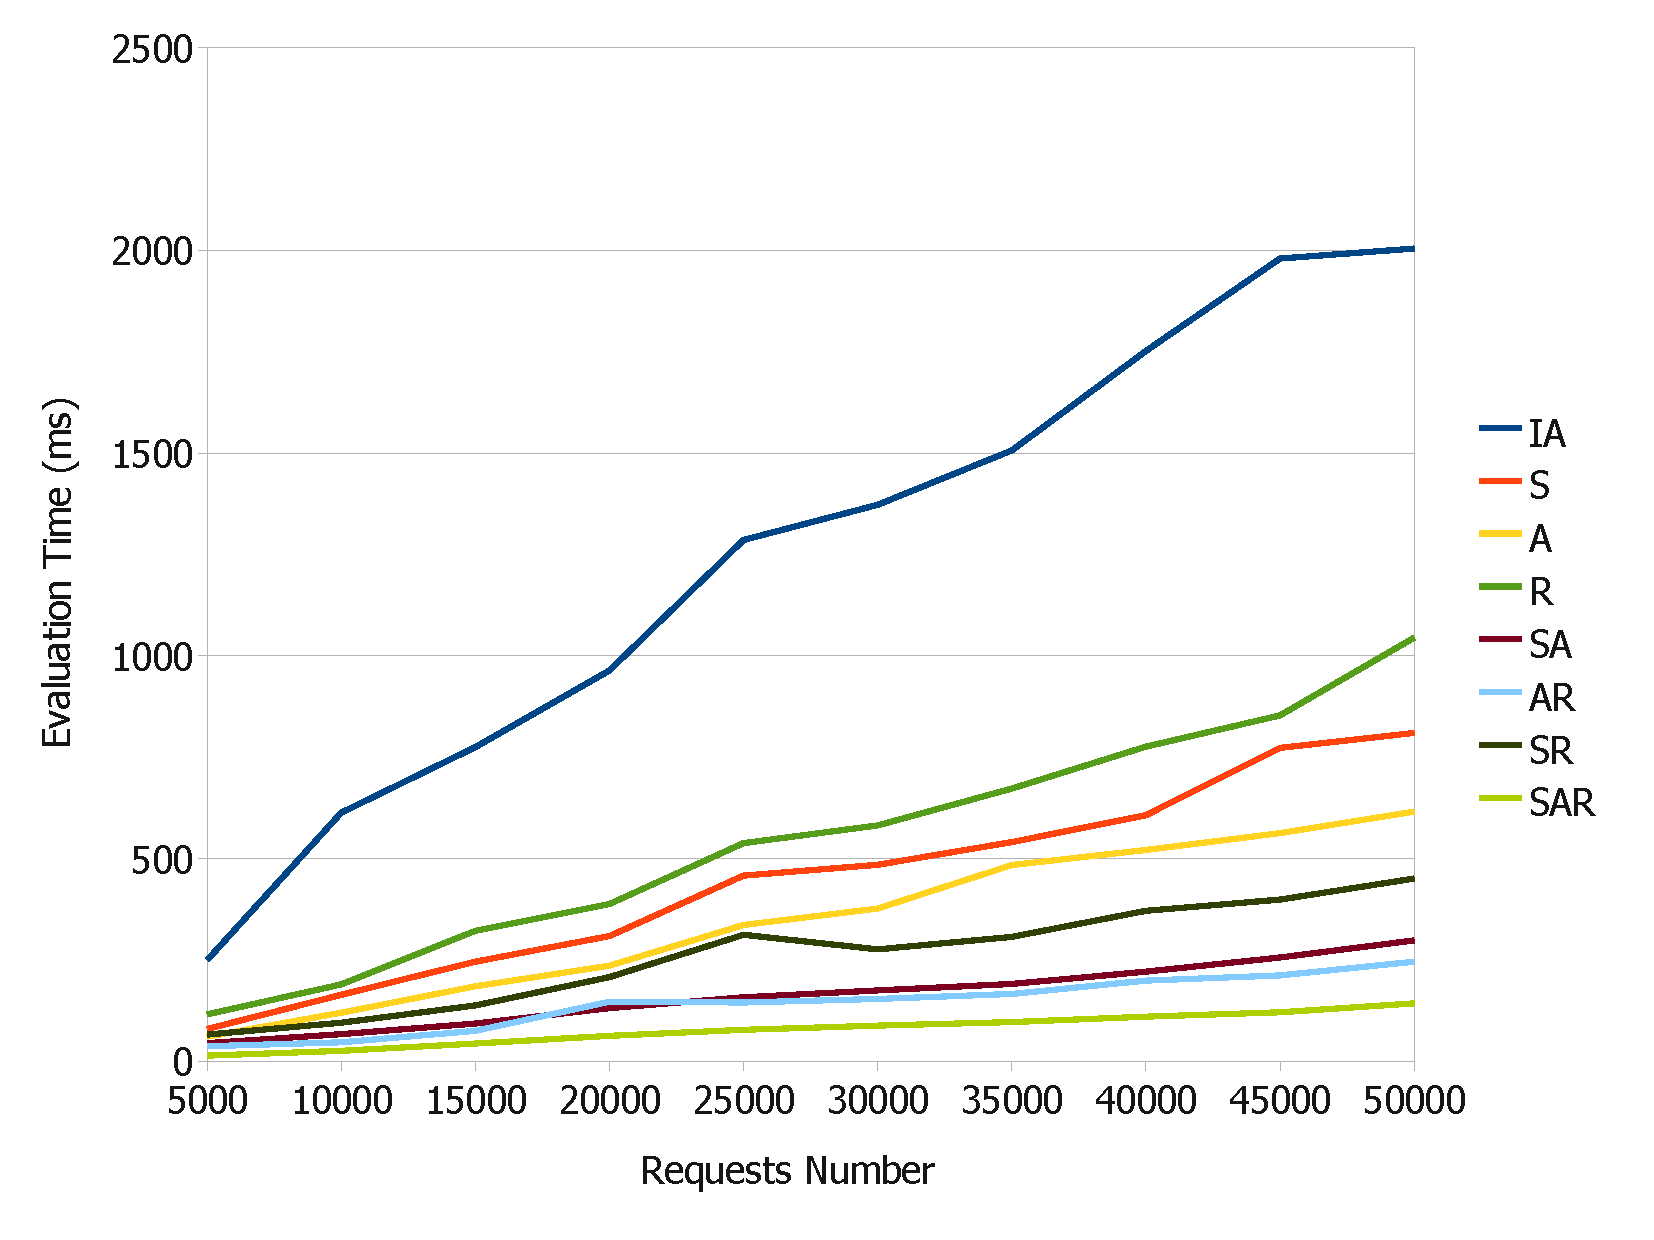
\includegraphics[width=0.34\textwidth]{X-LMS.pdf}}                
  \subfloat[VMS]{\label{fig:VMS}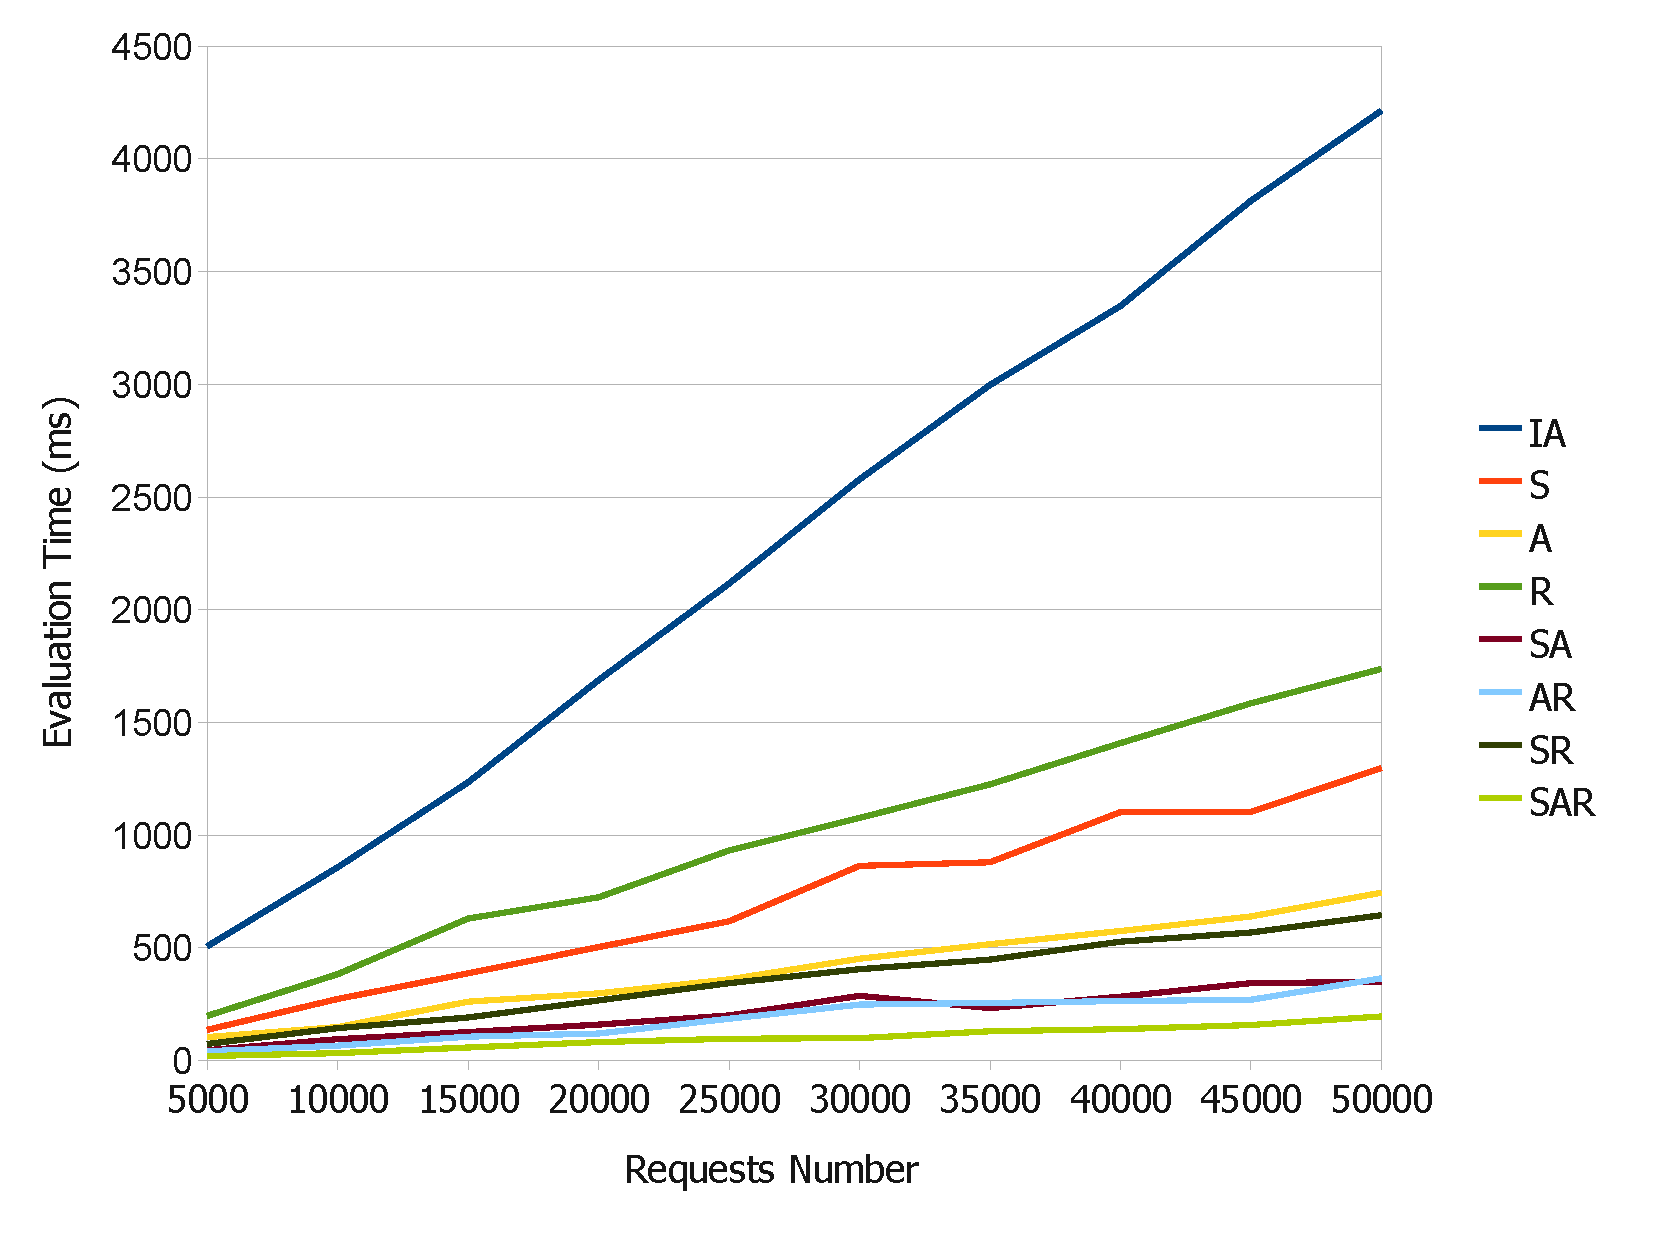
\includegraphics[width=0.34\textwidth]{X-VMS.pdf}}
  \subfloat[ASMS]{\label{fig:ASMS}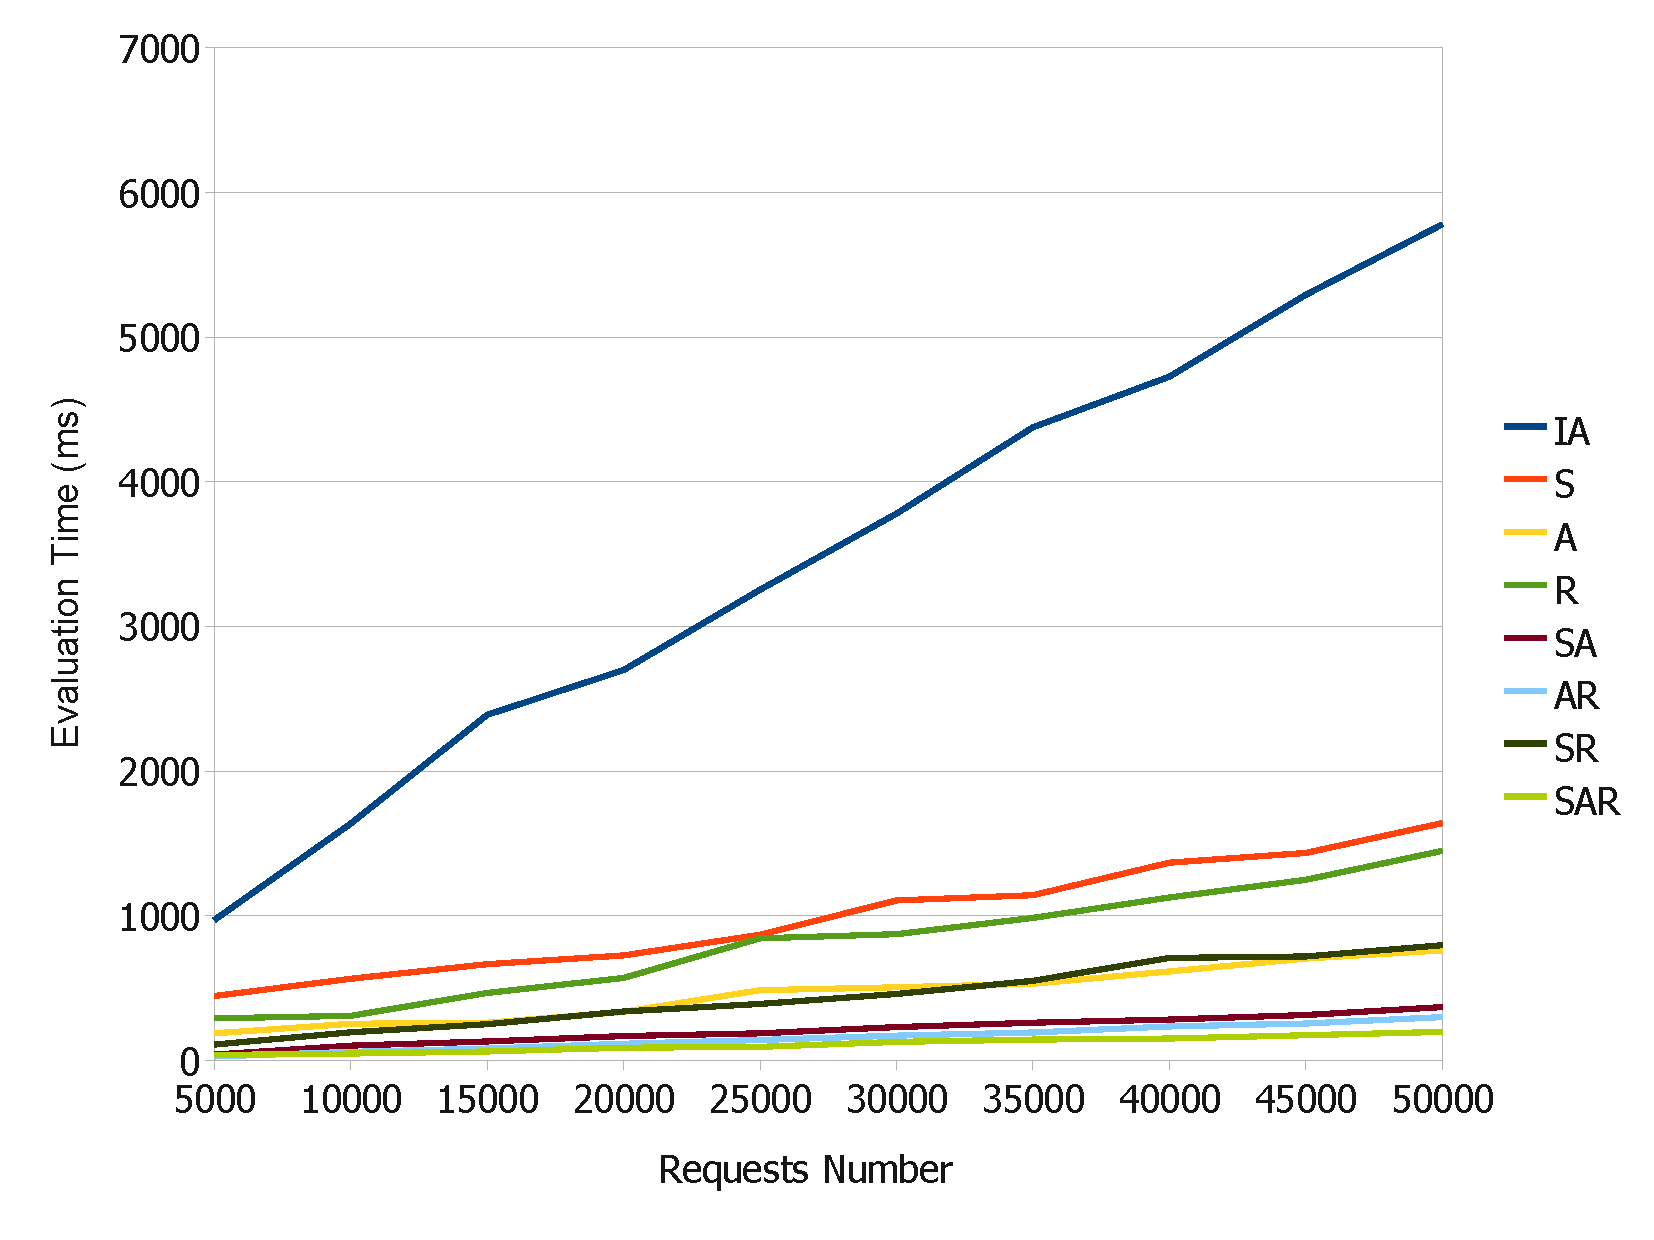
\includegraphics[width=0.34\textwidth]{X-ASMS.pdf}}
  \caption{Processing Time for our subjects, LMS, VMS and ASMS depending on the requests Number}
  \label{fig:processing time xengine}
\end{figure*}

To deploy our technique, we need to fetch the relevant PDP for a given request at runtime. Therefore, request processing time includes both fetching time and request evaluation time.
Figure \ref{Fetching Time} shows percentage of fetching time over the global evaluation time for request evaluation in LMS. 
The fetching time increases according to the PDP size. The fetching time is relatively small in comparison with the total evaluation time and thus 
does not impact significantly the decision making time.
\begin{figure}[!h]
  \centering
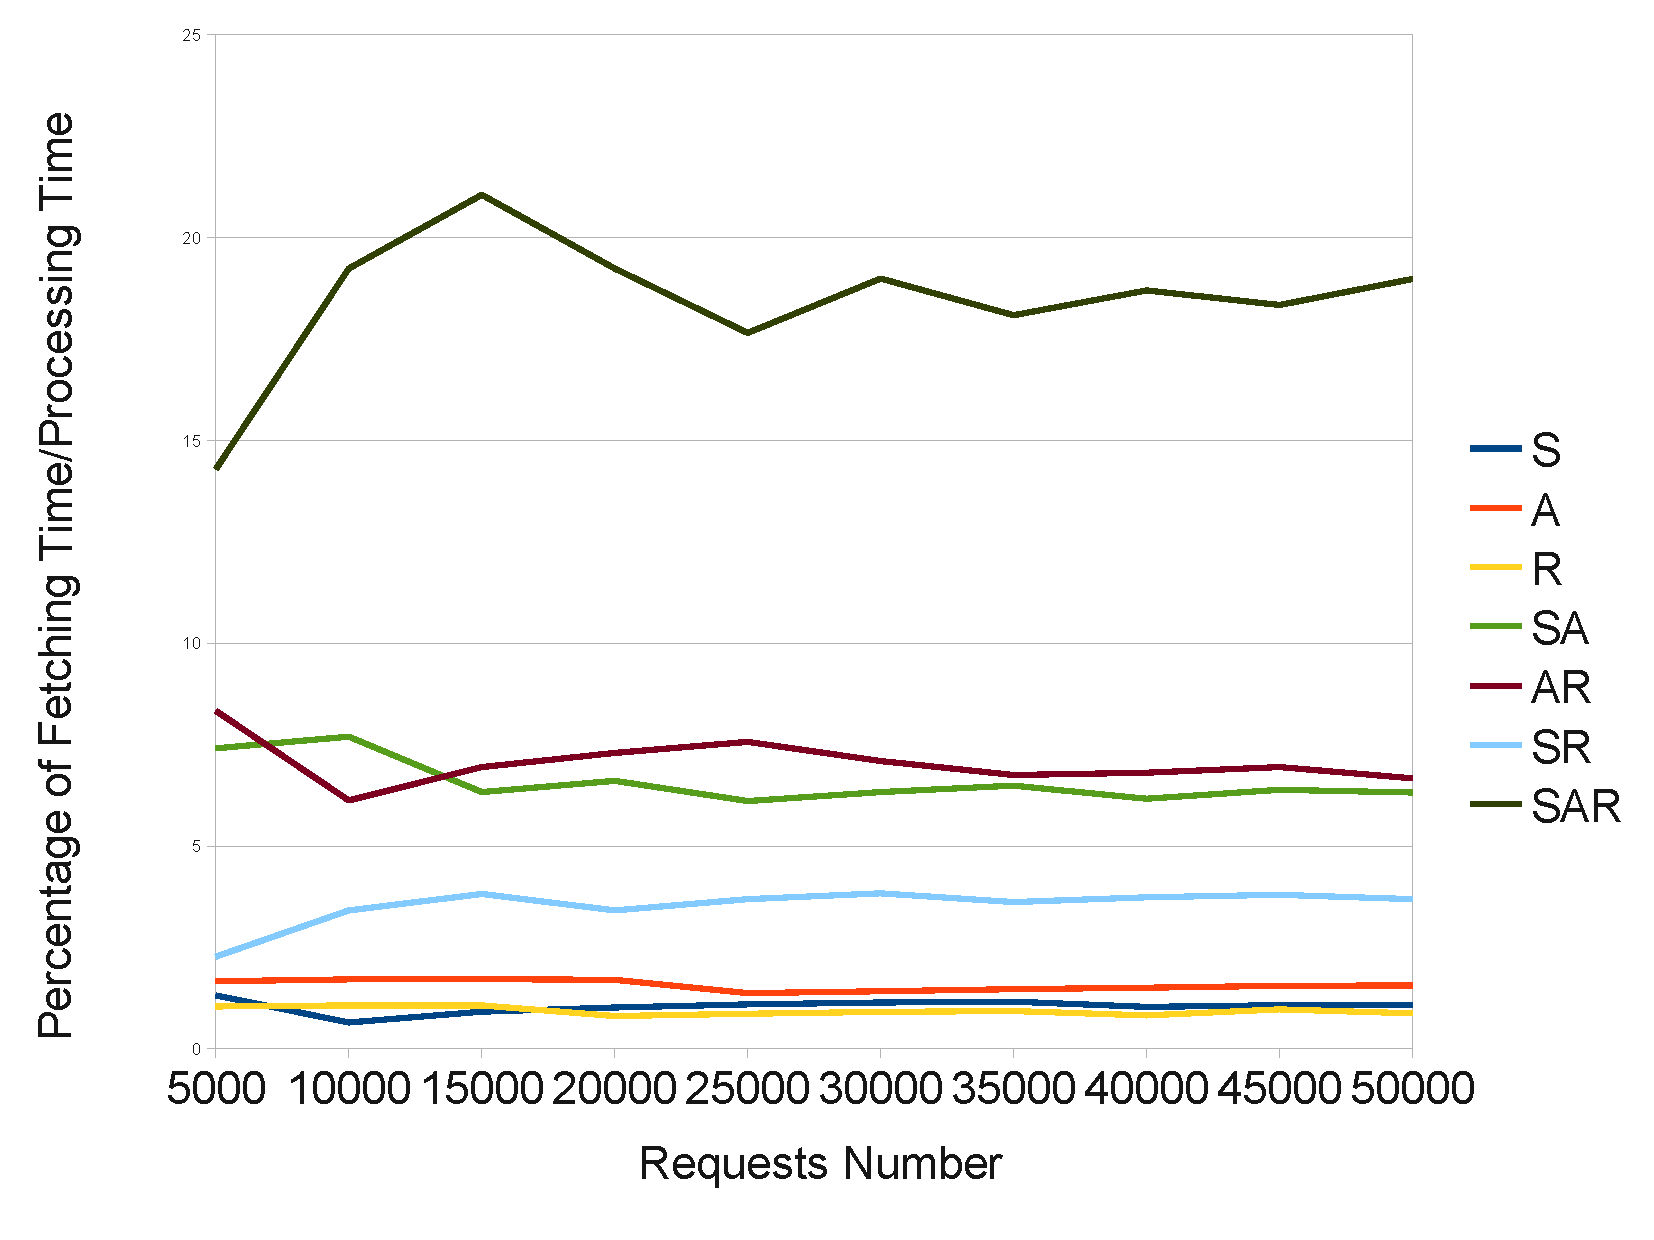
\includegraphics[width=8.5cm, height=7.2cm]{fetching.pdf}
\begin{center}
\caption{Percentage of Fetching Time}
\label{Fetching Time}
\end{center}
\end{figure}
\subsection{Summary}
We summarize the results of the evaluation section:
\begin{itemize}
 \item We have experimentally shown the effectiveness of the splitting in reducing the decision making time. Our refactoring process is more effective when 
it uses XEngine rather than Sun PDP to evaluate requests.
 \item When the sizes of PDPs are comparable, the splitting criteria that are synergic enable to have the best results in terms of 
decision making time.
\end{itemize}
The evaluation of the synergy property on improving performance has to be strengthened by conductinng others experiments 
on other evaluation studies and by considering different organizations of PEPs at the application level.
\subsection{Threats to Validity}
The threats to external validity primarily include the degree to which subjects, policies, splitting criteria and test requests are representative 
of true practice. These threats could be reduced by further evaluation on a wider type and larger number of subjects and policies and a larger number of 
test requests in future work. In particular, our approach is based on only seven proposed splitting criteria.  We could develop additional 
splitting criteria to split policies and measure efficiency in terms of request processing time. In addition, our approach generates random test requests, 
which may bias our results. To prevent such a bias, we conduct our evaluation for 10 times and measure an average value of evaluation results. 
The threats to internal validity are instrumentation effects that can bias our results such as faults in Sun PDP, XEngine, \CodeIn{PolicySplitter tool}, 
measurement tool in terms of request processing, and random request generators.
